\hypertarget{summary}{%
\section{Summary}\label{summary}}

MetaGenePipe (MGP) is an efficient, flexible, portable, and scalable
metagenomics pipeline that uses `best-in-domain' bioinformatics software
suites and genomic databases to create an accurate taxonomic
characterization of prokaryotic microbiome samples. Written in the
Workflow Definition Language (WDL), MGP produces output that is both
useful in its default form and can be used for further downstream
analysis. There are currently several contig-based taxonomic software
suites such as MG-RAST \autocite{keegan_glass_meyer_2016}, MMseqs2
\autocite{10.1093/bioinformatics/btab184}, and a few which make use of a
workflow language such as nf-core
\autocite{krakau_straub_gourle_gabernet_nahnsen_2022} (written in
Nextflow
\autocite{di_tommaso_chatzou_floden_barja_palumbo_notredame_2017}),
Muffin
\autocite{van_damme_hölzer_viehweger_müller_bongcam-rudloff_brandt_2021}
(Snakemake
\autocite{mölder_jablonski_letcher_hall_tomkins-tinch_sochat_forster_lee_twardziok_kanitz_et_al._2021}),
and Atlas \autocite{kieser_brown_zdobnov_trajkovski_mccue_2020}
(Nextflow). MGP is a pipeline-development best practice which uses
Singularity \autocite{kurtzer_sochat_bauer_2017} for containerization
and includes a setup script which downloads the necessary databases for
setup. The source code for MGP is freely available and is distributed
under the \href{https://www.apache.org/licenses/LICENSE-2.0}{Apache 2.0
license}.

The main advantage of MGP over MG-RAST is its ease of installation on
local infrastructure, requiring only the running of a setup script which
downloads a supplied Singularity image from SylabsCloud, the latest
version of Cromwell \autocite{voss_van_der_auwera_gentry_2022}, Koalafam
HMMER profiles
\autocite{aramaki_blanc-mathieu_endo_ohkubo_kanehisa_goto_ogata_2019},
and the Swiss-Prot database \autocite{uniprot_consortium_2018} which is
then converted to DIAMOND aligner \autocite{Buchfink2015-rn} format.
This setup allows MGP to be used across infrastructure and across
institutions.

The current software list includes the option of two genomic assemblers:
IDBA \autocite{peng_leung_yiu_chin_2012} and MegaHIT
\autocite{li_liu_luo_sadakane_lam_2015}, allowing for genomic assembly
in low-coverage samples or with high computational efficiency. The
included gene prediction tool, Prodigal (PROkaryotic Dynamic programming
Gen-finding Algorithm)
\autocite{hyatt_chen_locascio_land_larimer_hauser_2010}, is used to
predict gene coding sequences from raw genomic data. Alignment tools
incorporated into the workflow include DIAMOND,
\href{http://hmmer.org/}{HMMER}, and BLAST -- Basic Local Alignment
Search Tool --
\autocite{Camacho2009-hf,Altschul1990-xn,Altschul1997-oe}. These allow
for the alignment of predicted gene-coding sequences to known databases
for subsequent classification. Currently the Swiss-Prot database is used
for classifying genes to obtain protein descriptions and function.

MGP creates a taxonomic hierarchy classification using Kegg's Brite
hierarchy and KoalaFam HMMER profiles. MGP's focus can be modified to
find viruses, bacteria, plants, archaea, vertebrates, invertebrates, or
fungi by updating the reference databases to be kingdom specific.

\hypertarget{statement-of-need}{%
\section{Statement of need}\label{statement-of-need}}

Microorganisms such as bacteria, viruses, archaea, and fungi are
ubiquitous in our environment. The study of microorganisms and their
full genomes has been enabled through advances in culture independent
techniques and high-throughput sequencing technologies. Whole genome
metagenomics shotgun sequencing (WGS) empowers researchers to study
biological functions of microorganisms, and how their presence affects
human disease or a specific ecosystem. However, advanced and novel
bioinformatics techniques are required to process the data into a
suitable format. There is no universally accepted standardized
bioinformatics framework a microbiologist can use effectively.

MGP is written in WDL and thus differs from existing assembly-based
workflow pipelines such as Atlas (which uses Snakemake) and Muffin
(which is written in Nextflow). MGP is an example of WDL and
containerization best practice. Similar to NF-core/Mag, MGP employs
co-assembly as a feature. MGP differs from NF-Core as it has the option
to use IDBA, which is capable of assembling genomes from reads of uneven
sequencing coverage.

MGP overcomes traditional portability obstacles through the use of
Singularity containers and increases flexibility of research focus by
using the DIAMOND aligner --- able to create bespoke databases in a
matter of minutes. Researchers often have institutional datasets which
are a result of previous research. These datasets can be incorporated
into MGP in place of the default DIAMOND and BLAST databases. Once these
databases have been created, an update in the relevant line in the
configuration file will allow the workflow to use the new database.
While MGP is focussed on prokaryotes, it can easily be adapted to
eukaryotes or viruses by changing the prokaryotic gene prediction
software, Prodigal, to a eukaryotic gene prediction software such as
GeneMark-EP+ \autocite{10.1093/nargab/lqaa026},
\href{http://eugene.toulouse.inra.fr/}{EuGene} \autocite{Sallet2019} for
eukaryotes or a gene finding tool for viruses.

\begin{figure}
\centering
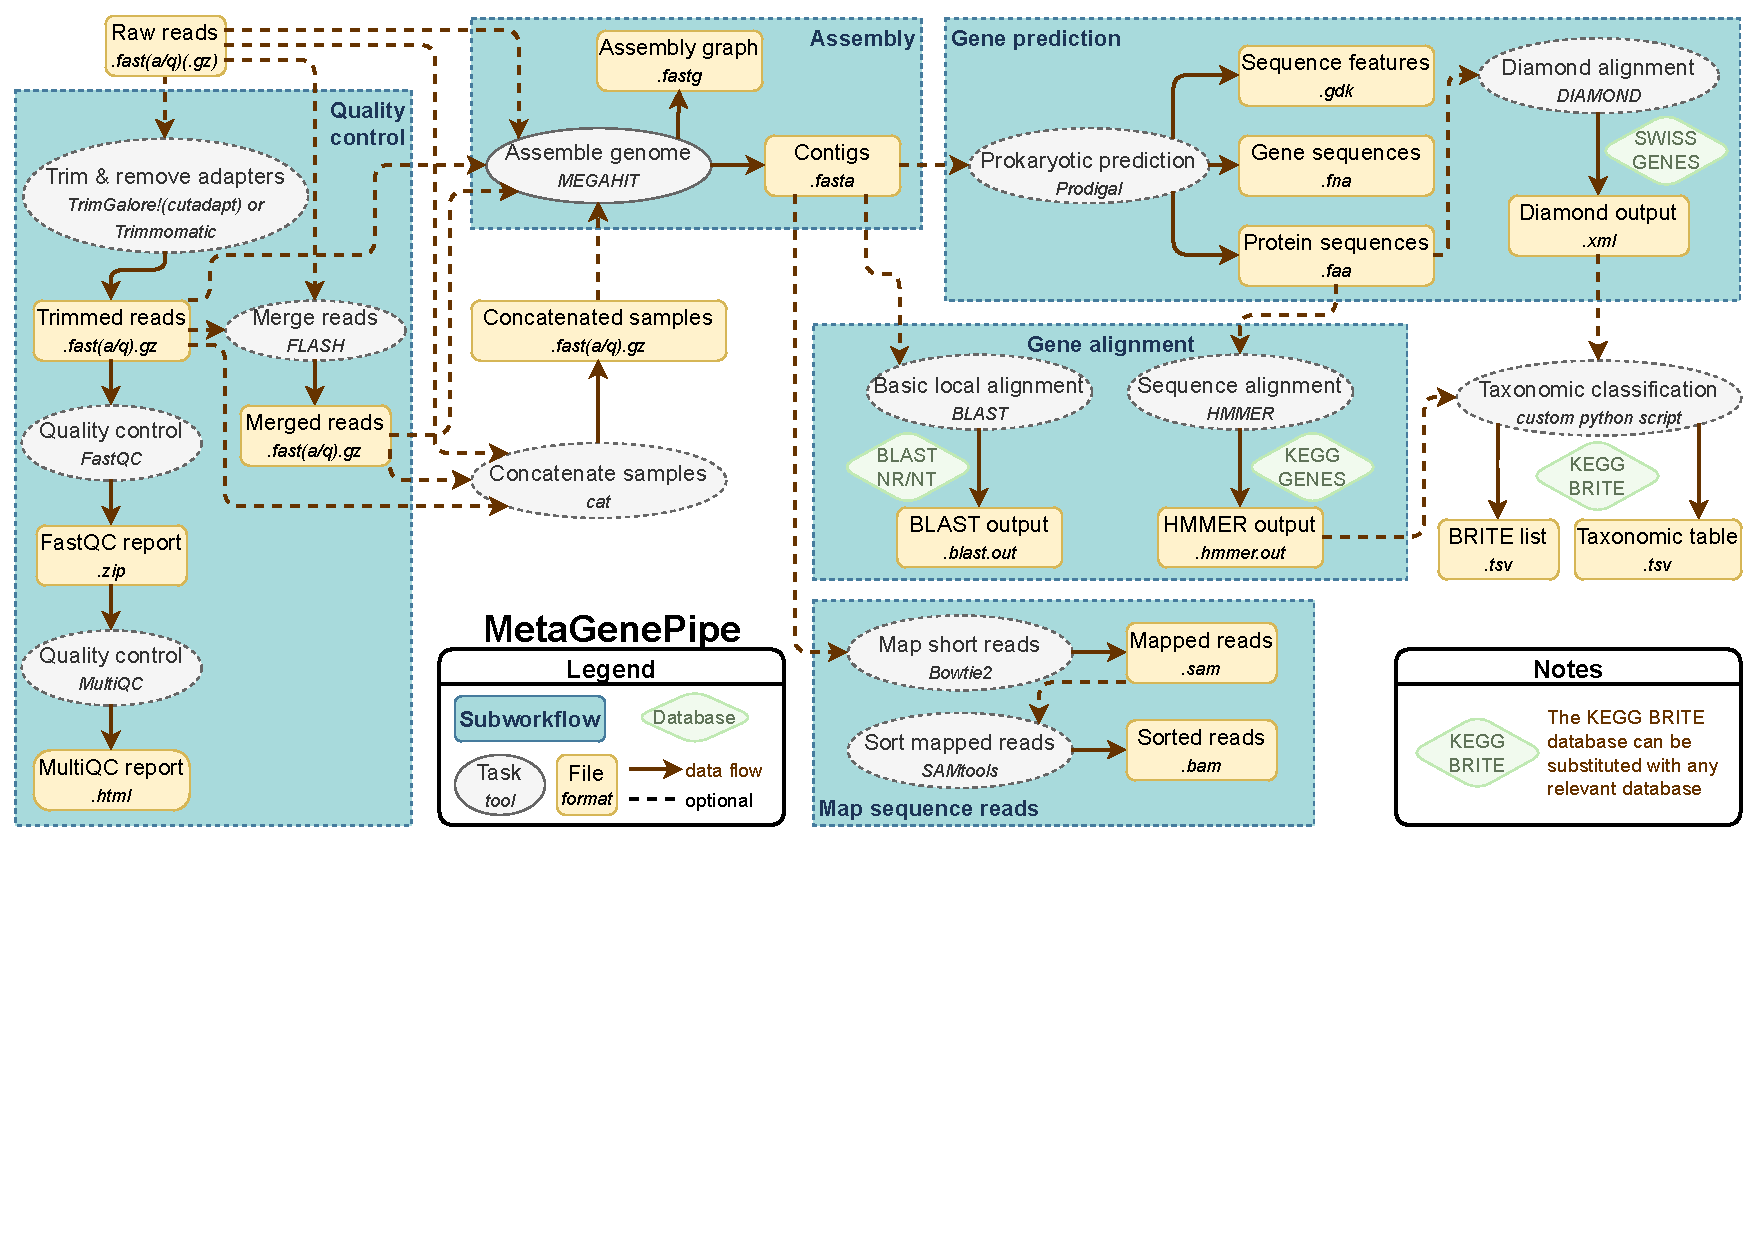
\includegraphics{logo/MetaGenePipe.drawio.pdf}
\caption{The MetaGenePipe Workflow}
\end{figure}

\hypertarget{workflow}{%
\section{Workflow}\label{workflow}}

MGP is written in the \href{https://openwdl.org/}{Workflow Definition
Language (WDL)} which is renowned for specifying data processing
workflows in human-readable and writable syntax. Singularity is used to
containerize the required software for MGP to run and is stored in
\href{https://sylabs.io/}{SylabsCloud} for universal accessibility.

MGP is broken up into three sub-workflows: Quality Control (QC),
Assembly, and Gene Prediction. Each subworkflow contains related tasks
that are necessary for that portion of the workflow.

\hypertarget{qc-sub-workflow}{%
\subsection{QC Sub-workflow}\label{qc-sub-workflow}}

The quality control (QC) sub-workflow allows the trimming of genomic
samples for poor quality reads and any adapter sequence which may be
present via the use of either Trimmomatic \autocite{pmid24695404} or
TrimGalore \autocite{felix_krueger_2021_5127899}. There is also the
option of merging the reads by merging overlapping reads paired-end
reads using FLASH \autocite{Magoc2011-gb}. Lengthening reads (via
merging with FLASH) can help overcome potential low-coverage regions
encountered during the assembly process. Visualizations of the sequence
quality are obtained using FastQC \autocite{Andrews:2010tn} and the
subsequent FastQC output is merged and analyzed as a whole using MultiQC
\autocite{10.1093/bioinformatics/btw354}.

\hypertarget{concatenate-samples}{%
\subsection{Concatenate Samples}\label{concatenate-samples}}

This is a standalone task that allows for the option of concatenating
samples by merging forward reads and reverse reads into files combining
all available samples. This step is intended to facilitate co-assembly
of the available sequences. Co-assembly has shown to provide more
complete genomes, with lower error rates when compared to multiassembly
\autocite{hofmeyr2020}.

\hypertarget{assembly-sub-workflow}{%
\subsection{Assembly sub-workflow}\label{assembly-sub-workflow}}

The Assembly sub-workflow includes two genomic assemblers: IDBA and
MegaHIT. IDBA is known for being able to assemble genomic samples with
uneven sequencing length \autocite{10.1093/bioinformatics/bts174}, while
MegaHIT performs de-novo assembly of large and complex metagenomic
samples in a time and cost-efficient manner
\autocite{10.1093/bioinformatics/btv033}.

\hypertarget{gene-prediction-sub-workflow}{%
\subsection{Gene Prediction
sub-workflow}\label{gene-prediction-sub-workflow}}

The gene prediction sub-workflow uses Prodigal for the prediction of
prokaryotic gene coding sequences and identifying the sites of
translation initiation \autocite{Hyatt2010-zh}. Prodigal produces an
\texttt{fna} file with the resulting protein prediction. The predicted
gene coding sequences are then aligned to the Swiss-Prot database
\autocite{pmid18287689} with the \mbox{DIAMOND} Aligner and to
\href{https://www.genome.jp/tools/kofamkoala/}{KoalaFam HMMER profiles}
\autocite{pmid31742321}. Custom Python scripts are then used to extract
the output of the alignments and match genes to functional hierarchies
using the \href{https://www.genome.jp/kegg/brite.html}{KEGG Brite
Database} \autocite{pmid10592173,pmid31441146,pmid33125081}.

\hypertarget{read-mapping-and-blast}{%
\subsection{Read Mapping and BLAST}\label{read-mapping-and-blast}}

Aligning raw reads back to the assembled contigs has the advantage of
discerning the relative abundance of contigs in a metagenomics dataset.
This is an important step in downstream genomic binning and metagenome
statistics. The raw reads that have passed the QC stage are at this
point aligned back to the contigs that are the output of the assembly
sub-workflow using the Burrows-Wheeler Aligner (BWA)
\autocite{Li2010-nl}. A compressed binary file representing the
alignment of raw sequences to the assembly output in BAM format is
created via BamTools \autocite{10.1093/bioinformatics/btr174} and
analysis performed using SAMtools's
\autocite{10.1093/bioinformatics/btp352} flagstat function to determine
the percentage of raw reads that were used for the assembly.

BLAST is used to query the contigs created during assembly against the
NCBI NT/NR database to determine which species the assembled contigs
belong to. The BLAST output is parsed in such a way that it is easily
searchable and still lists queries which return no hits. This allows
researchers to extract these potentially novel results for further
investigation. Additionally, the BLAST results can be used to filter
contigs that belong to a taxonomy of interest which do not provide a
match during the Swiss-Prot alignment stage for the purposes of genomic
binning or targeted investigation for regions of interest.

\hypertarget{resource-usage-and-infrastructure-requirements}{%
\subsection{Resource Usage and Infrastructure
requirements}\label{resource-usage-and-infrastructure-requirements}}

MGP relies on Unix's \texttt{time} tool to measure the resources that
each task uses, such as CPU usage, file size, elapsed time, and system
time. This output can be parsed to create visualizations that can be
used in deciding resource requests for the workflow when executing it
using a job scheduler on high-performance computing infrastructure.
Table 1 shows the resource usage for processing paired-end samples of
25,000 reads each. Table 2 shows the resource usage for running Cromwell
on the head node.

MGP can be run locally on a laptop, a virtual machine, or in a
high-performance computing setting.

\begin{longtable}[]{@{}
  >{\raggedright\arraybackslash}p{(\columnwidth - 6\tabcolsep) * \real{0.2000}}
  >{\raggedright\arraybackslash}p{(\columnwidth - 6\tabcolsep) * \real{0.3368}}
  >{\raggedright\arraybackslash}p{(\columnwidth - 6\tabcolsep) * \real{0.2105}}
  >{\raggedright\arraybackslash}p{(\columnwidth - 6\tabcolsep) * \real{0.2526}}@{}}
\toprule
\begin{minipage}[b]{\linewidth}\raggedright
Task
\end{minipage} & \begin{minipage}[b]{\linewidth}\raggedright
User Time (mm:ss)
\end{minipage} & \begin{minipage}[b]{\linewidth}\raggedright
CPU utilization
\end{minipage} & \begin{minipage}[b]{\linewidth}\raggedright
Max Memory (kbytes)
\end{minipage} \\
\midrule
\endhead
fastqc & 00:04.0 & 226\% & 233376 \\
flash & 00:00.3 & 129\% & 13140 \\
trim\_galore & 00:02.30 & 183\% & 22772 \\
diamond & 00:03.2 & 477\% & 392904 \\
hmmer & 03:06.4 & 104\% & 39296 \\
prodigal & 00:00.4 & 96\% & 49088 \\
blast & 01:30.1 & 188\% & 13308876 \\
megahit & 00:08.2 & 446\% & 66944 \\
multiqc & 00:04.5 & 84\% & 78084 \\
read alignment & 00:02.0 & 117\% & 91952 \\
\bottomrule
\end{longtable}

Table 1: The resource usage for processing paired end samples of 25,000
reads each in MetaGenePipe.

\begin{longtable}[]{@{}
  >{\raggedright\arraybackslash}p{(\columnwidth - 6\tabcolsep) * \real{0.2000}}
  >{\raggedright\arraybackslash}p{(\columnwidth - 6\tabcolsep) * \real{0.3368}}
  >{\raggedright\arraybackslash}p{(\columnwidth - 6\tabcolsep) * \real{0.2105}}
  >{\raggedright\arraybackslash}p{(\columnwidth - 6\tabcolsep) * \real{0.2526}}@{}}
\toprule
\begin{minipage}[b]{\linewidth}\raggedright
Task
\end{minipage} & \begin{minipage}[b]{\linewidth}\raggedright
User Time (mm:ss)
\end{minipage} & \begin{minipage}[b]{\linewidth}\raggedright
CPU utilization
\end{minipage} & \begin{minipage}[b]{\linewidth}\raggedright
Max Memory (kbytes)
\end{minipage} \\
\midrule
\endhead
fastqc & 08:50.9 & 12\% & 57280 \\
\bottomrule
\end{longtable}

Table 2: The resource usage for running Cromwell on the head node.

\hypertarget{acknowledgements}{%
\section{Acknowledgements}\label{acknowledgements}}

We thank the members of the Verbruggen lab, Kshitij Tandon and Vinicius
Salazar in particular, for sharing ideas, feedback, and testing the
workflow. This research was supported by The University of Melbourne's
Research Computing Services and the Petascale Campus. The project
benefited from funding by the Australian Research Council (DP200101613
to Heroen Verbruggen).
